\section{Appendix}

\begin{table}[h]
\centering
\captionsetup{singlelinecheck=false, justification=centering}
\caption{Summary statistics for nominal and real rates (annualized rates) \\ \cite{collard11} sample (1960:I to 2006:IV)}
\label{implied-vs-ffr-nipa-collard}
\begin{tabular}{lccccc} \hline
& Data & SEP & SEP + HP & NSEP & NSEP + HP \\ \hline
\multicolumn{6}{c}{Real interest rates} \\ \hline
\csvreader[head to column names, late after line = \\]%
  {tables/nipa/collard-real.csv}{}%
  {\stat & \data & \sep & \sephp & \nsep & \nsephp} \hline
\multicolumn{6}{c}{Nominal interest rates} \\ \hline
\csvreader[head to column names, late after line = \\]%
  {tables/nipa/collard-nominal.csv}{}%
  {\stat & \data & \sep & \sephp & \nsep & \nsephp} \hline
\end{tabular}
\end{table}

\begin{figure}[h]
\ContinuedFloat*
\centering
\begin{tabular}{cc}
Real rates ($\rho = -0.050$) & Nominal rates ($\rho = 0.142$) \\
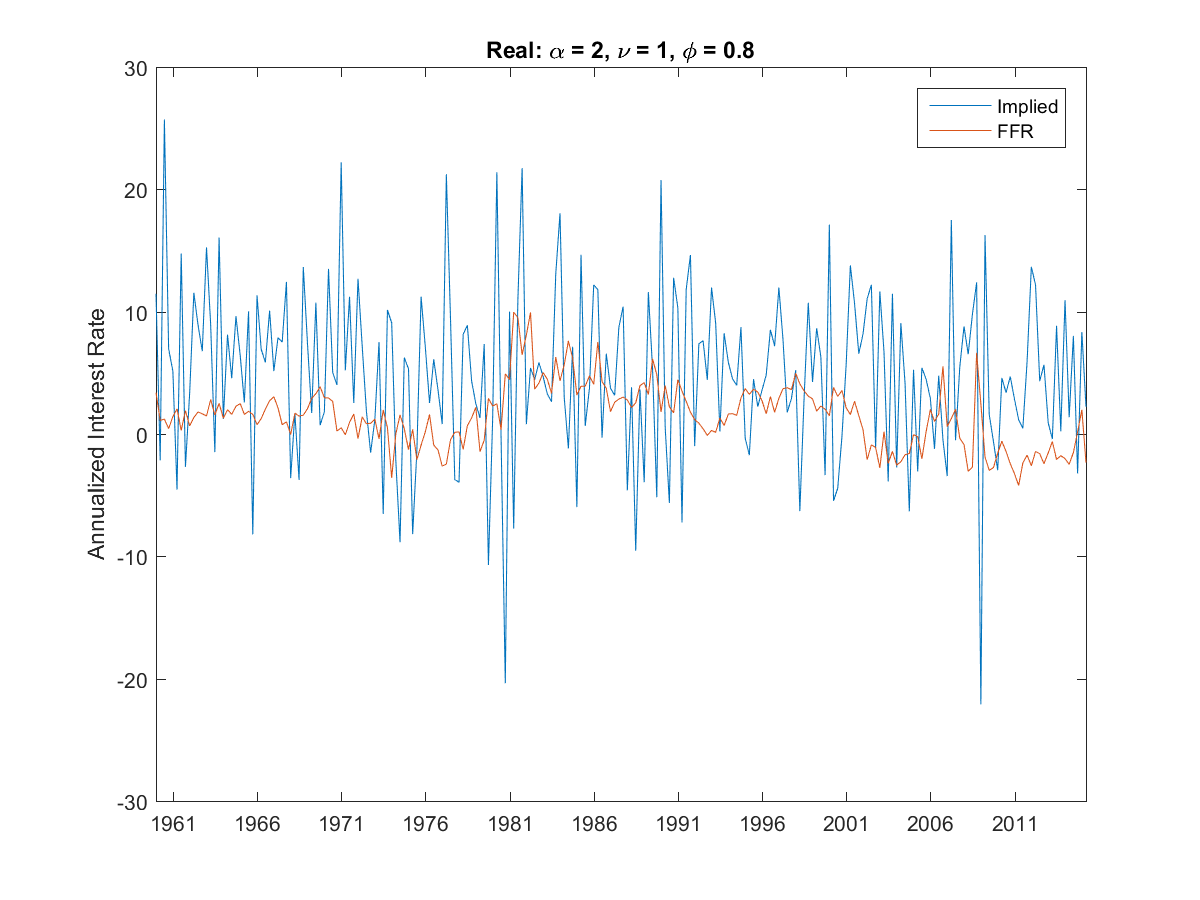
\includegraphics[width=0.49\textwidth]{figs/nipa/implied-vs-ffr/real_sep-hp} &
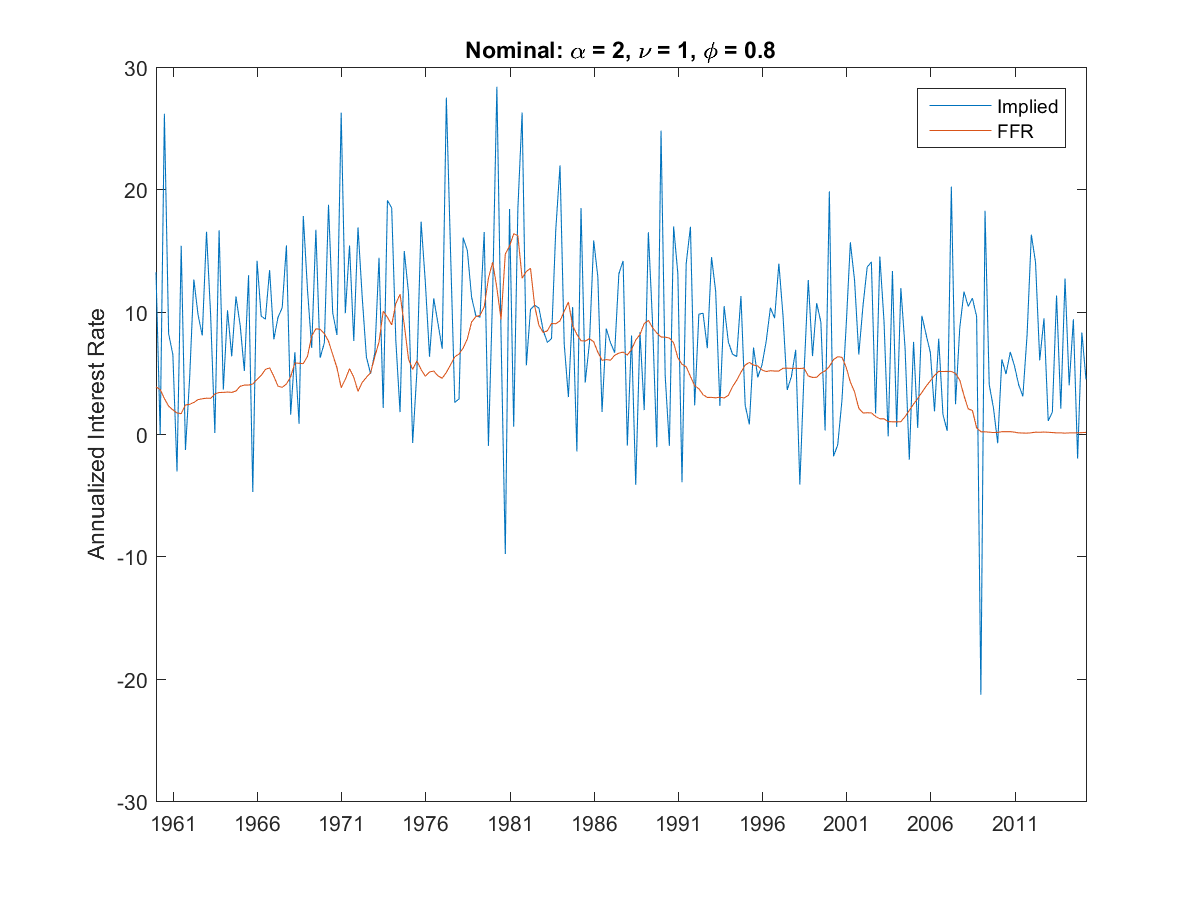
\includegraphics[width=0.49\textwidth]{figs/nipa/implied-vs-ffr/nominal_sep-hp}
\end{tabular}
\caption{SEP + HP implied vs. observed rates}
\label{implied-vs-ffr-nipa-others}
\end{figure}

\begin{figure}[h]
\ContinuedFloat
\centering
\begin{tabular}{cc}
Real rates ($\rho = 0.261$) & Nominal rates ($\rho = 0.707$) \\
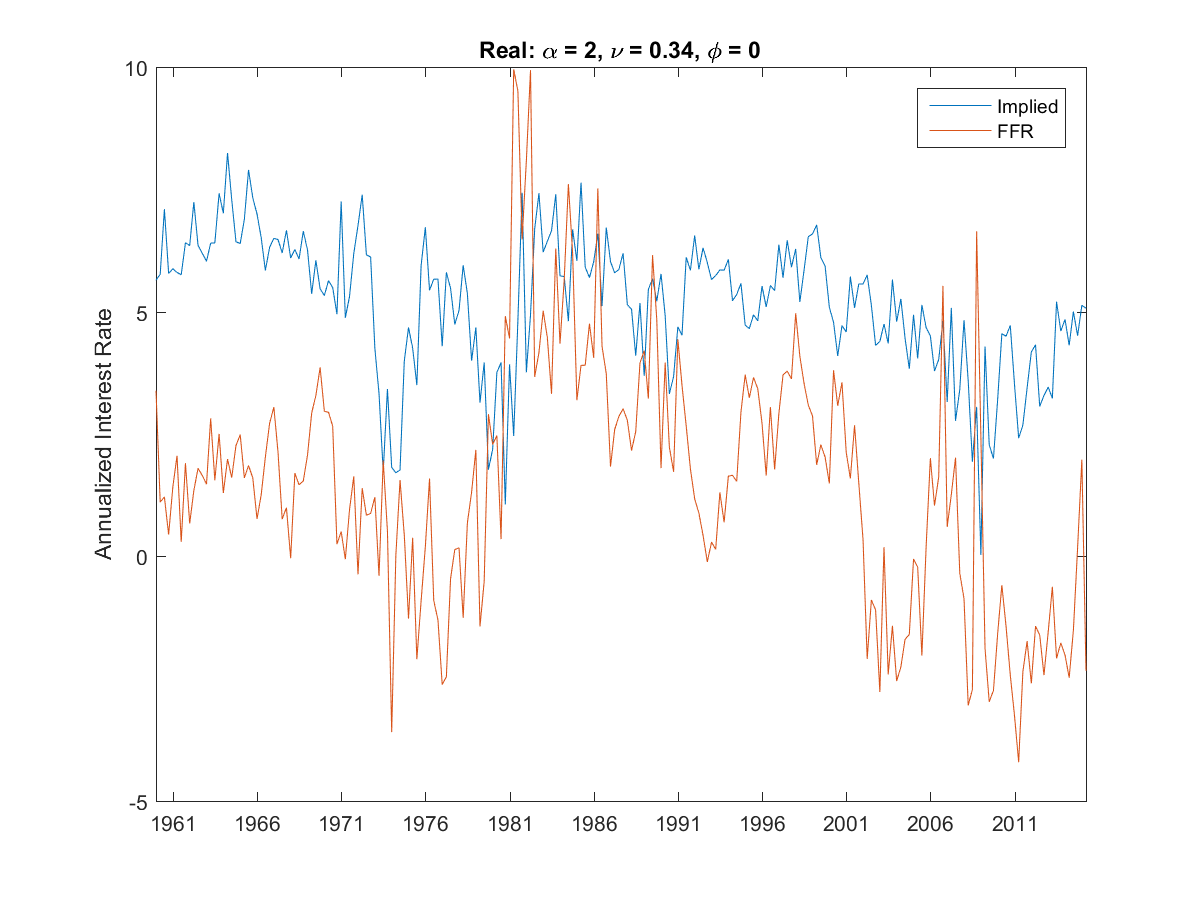
\includegraphics[width=0.49\textwidth]{figs/nipa/implied-vs-ffr/real_nsep} &
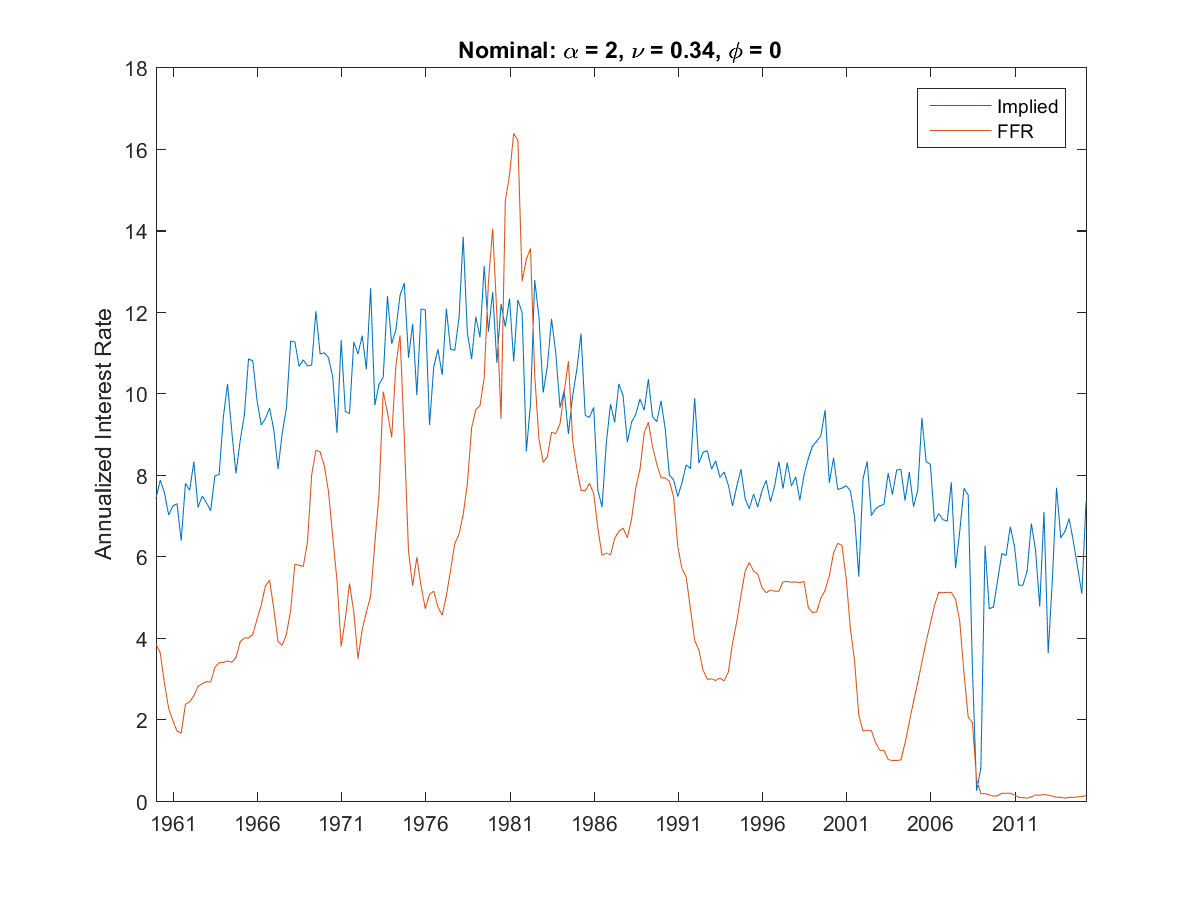
\includegraphics[width=0.49\textwidth]{figs/nipa/implied-vs-ffr/nominal_nsep}
\end{tabular}
\caption{NSEP  implied vs. observed rates}
\end{figure}

\begin{figure}[h]
\ContinuedFloat
\centering
\begin{tabular}{cc}
Real rates ($\rho = 0.033$) & Nominal rates ($\rho = 0.390$) \\
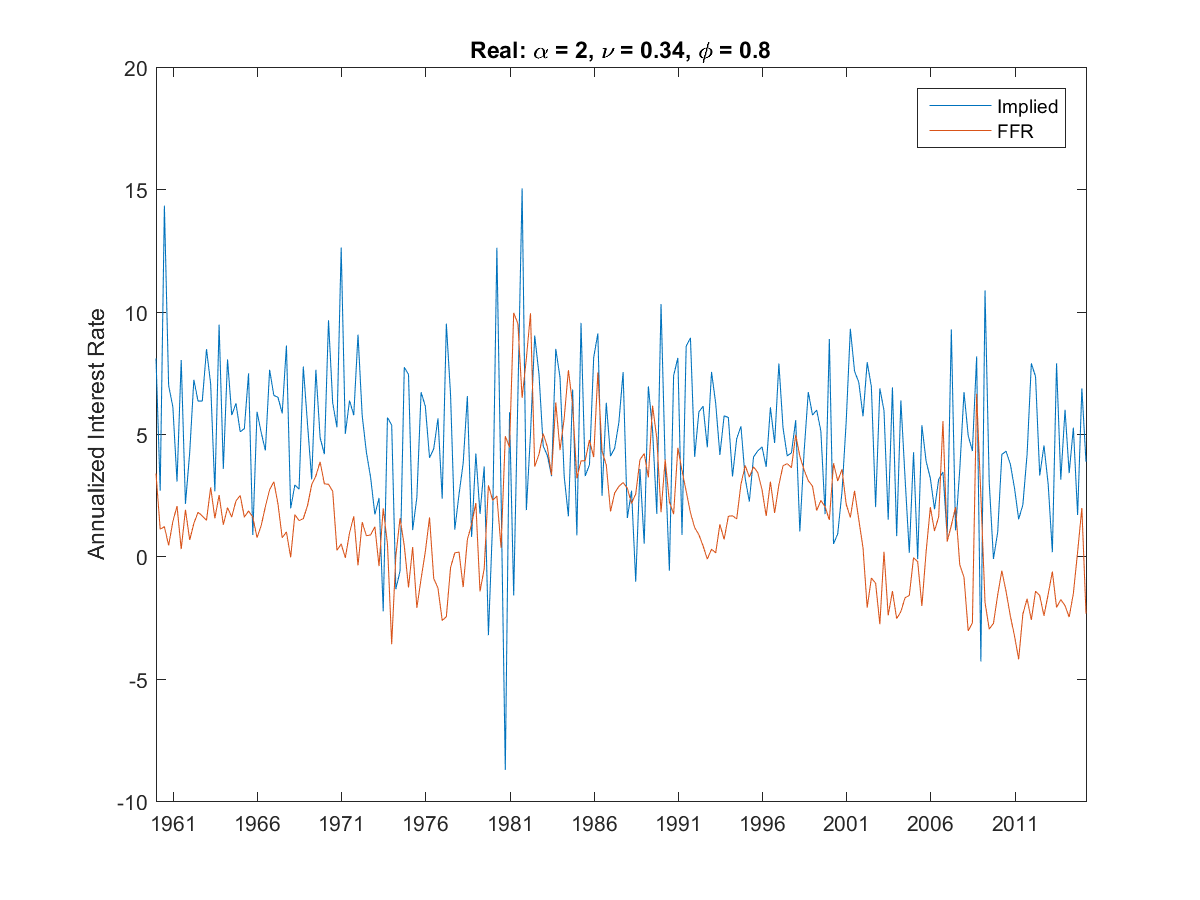
\includegraphics[width=0.49\textwidth]{figs/nipa/implied-vs-ffr/real_nsep-hp} &
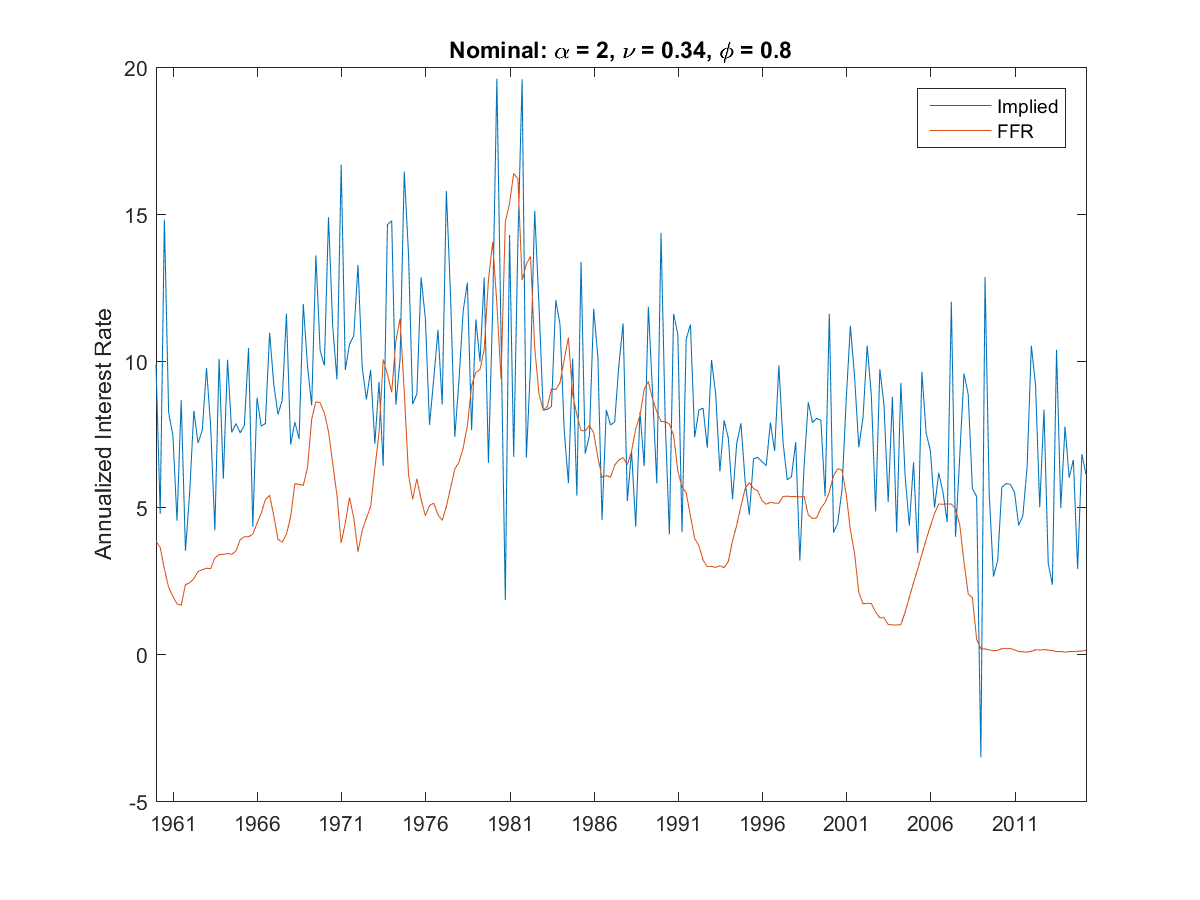
\includegraphics[width=0.49\textwidth]{figs/nipa/implied-vs-ffr/nominal_nsep-hp}
\end{tabular}
\caption{NSEP + HP implied vs. observed rates}
\end{figure}

\begin{table}[h]
\centering
\caption{Comparison of responses of spread to monetary policy \\ (Standard errors in parentheses)}
\label{spread-comparison-nipa}
\begin{tabular}{lcccccc} \hline
                   & SEP     & SEP + HP & NSEP    & NSEP + HP & Start  & End \\ \hline
\multicolumn{7}{c}{Real interest rate spreads} \\ \hline
Full Sample        & -0.307  & -0.906   & -0.312  & -0.623    & 1960:I & 2015:II \\
                   & (0.050) & (0.165)  & (0.044) & (0.093) \\
Restricted Sample  & -0.545  & -1.054   & -0.432  & -0.734    & 1966:I & 2003:IV \\
                   & (0.069) & (0.226)  & (0.057) & (0.130) \\
\cite{canzoneri07} & -0.482  & -1.215   & ---     & ---       & 1966:I & 2003:IV \\ 
                   & (0.064) & (0.825) \\\hline
\multicolumn{7}{c}{Nominal interest rate spreads} \\ \hline
Full Sample        & -0.273  & -0.954   & -0.282  & -0.640    & 1960:I & 2015:II \\
                   & (0.043) & (0.161)  & (0.036) & (0.089) \\
Restricted Sample  & -0.545  & -1.134   & -0.433  & -0.796    & 1966:I & 2003:IV \\
                   & (0.064) & (0.223)  & (0.050) & (0.128) \\
\cite{canzoneri07} & -0.357  & -1.035   & ---   & ---       & 1966:I & 2003:IV \\ 
                   & (0.047) & (0.826) \\\hline
\end{tabular}
\end{table}
